\documentclass[10pt,twoside,dutch,english]{report}

    \usepackage[times]{quotchap}   % fancy chapter beginning
    \usepackage{fancyhdr}
	\usepackage[justification=raggedright, font=small, labelfont=bf,singlelinecheck=false]{caption}     %better control over captions (sideways, font, ...)  
    \usepackage{subfigure}  % with scriptsize or so, one can adapt the size


    \usepackage{enumerate}  % to make it possible to define the numbers (A,a, ...)
   % \usepackage{psfrag}
    \usepackage{graphicx}
    
    %tables
    \usepackage{tabu} %table package. Veel mogelijkheden, bomen en bos
    \usepackage{mbenotes}
    \usepackage{tabularx}

 
    \usepackage{threeparttable} %tables with notes
       \usepackage[referable]{threeparttablex}
    %\usepackage[table]{xcolor}
  
	 \usepackage{booktabs}
   \usepackage{array}
  

    
    
    \usepackage{csvsimple} % csv inladen. Werkt nog niet
    %\usepackage{datatool}
    \usepackage{hyperref}
    \hypersetup{
    	colorlinks,
    	citecolor=dimgray,
    	filecolor=black,
    	linkcolor=black,
    	urlcolor=black
    }
    \definecolor{dimgray}{rgb}{0.41, 0.41, 0.41}
    
    \usepackage[toc,page]{appendix}
    
   % \usepackage{chappg}     % page numbering (chapno-pageno), for ToC
    \usepackage{url}        % for better url typesetting
    \usepackage{hhline}     % generates nicer table lines (without missing pixels) + more flexible
    \usepackage{afterpage}  % adds \afterpage command, which makes it possible to issue \afterpage{\clearpage} which flushes all floats after this page
    
    \usepackage[version = 4]{mhchem}     % use \ce {}  for chemical forumals
    \usepackage[a4paper]{geometry}
    \usepackage{fullpage}
    \usepackage{cmbright}
    % \usepackage{cm-super}
    % \usepackage{microtype} %geeft nog een error

   \usepackage[round]{natbib}

\author{Job de Pater}
\title{Linking nitrogen mineralization to forage production} % was eerst anders.

\begin{document}
\maketitle


\setcounter{tocdepth}{1}
\tableofcontents

\thispagestyle{empty}
\pagebreak
\pagenumbering{arabic}

%\chapter*{Summary}

%\chapter*{Preface}

\chapter{Introduction}
%Voor 80% af op 10/7/15
The goal of this project is to get more insight in soil processes that influence the relation between soil quality and forage production. Focus of this study is on the general research pattern. 

	\section{Relevance}
	We want to grow more forage with less fertilization. Nitrogen (N) is often growth limiting, partly because of the more and more strict regulations on fertilizer and manure application. Mineralization of soil organic matter (SOM) is a key soil process, a.o. because it provides the plants with mineral N. To maintain yields and prevent losses (leaching, volatilization) a balanced nitrogen management is required. It is increasingly important to give farmers clear soil management guidelines. Much is known on the nutrient behavior in soils. However, all this knowledge has to be put into practice. Farmers has to know the target range in what certain meaningful indicators has to felt in to optimize yields and maintain a good soil quality. Therefore, relations between soil indicators and forage production has to be investigated to study the SOM behavior and to upgrade soil N fertilization recommendations. 
	
	
		\section{Background} %De aanleiding voor het onderzoek
	
			
		\subsection{Nutrient flows in grass production}
		The efficiency of forage production in terms of nutrient in- and outputs becomes more and more important in modern dairy farming. Forage production depends among others on soil quality, fertilization and other pasture management actions. It is known that fertilization practices affects the structure and composition of herbage directly, but there are not much studies that links soil fertility with herbage quality under practical conditions \citep{Reijneveld2014}. In terms of farm nutrient management, the aim is to distribute the available amount of fertilizer and manure in the most efficient way. Therefore, the nutrient usage as well as the SOM mineralization has to be considered over time. It will also pay of in nutrient use efficiency to consider spatial differences in soils in order to distribute the nutrients most advantageous over all fields within a farm.  A first step is the development of the instrument Annual Nutrient Cycling Assessment (ANCA, dutch: 	\href{http://www.wageningenur.nl/nl/show/KringloopWijzer-2.htm}{\textit{Kringloopwijzer}}). The ANCA instrument is developed to presents a clear overview of individual farm nutrient cycles \citep{Aarts2013}. All nutrient flows can be described by existing data of the whole farm (Figure \ref{fig:KLW}). This tool has high potential for governmental regulations, farm management advices and it provides knowledge and data for fundamental and applied research. However, a big disadvantage of the ANCA system is that the soil part is not yet implemented. There are no thoroughly computation rules for translating soil quality in forage production and vice versa. This lack of data causes a gap in the ANCA model and influences the outcome of the balance. 
		
		\begin{figure}[ht]
			\centering
			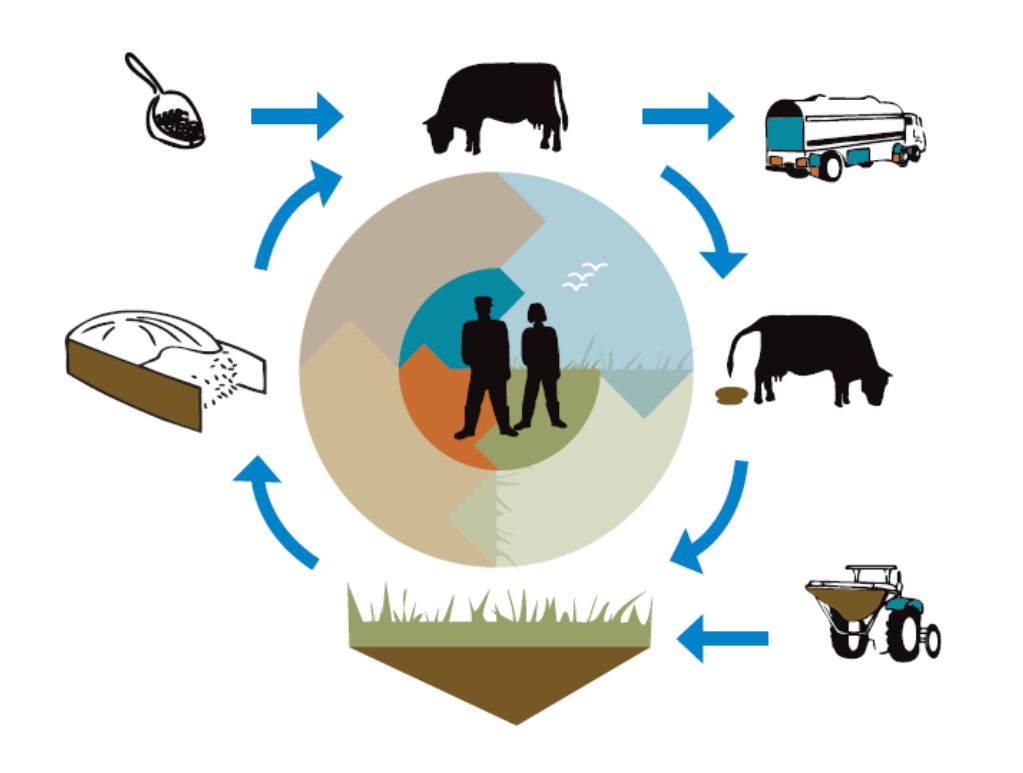
\includegraphics[width=0.6\linewidth]{intro_KLW}
			\caption{The different parts of the ANCA instrument: animal, forage, milk, fertilization and soil. Data for the instrument is provided by certain companies. The relations between fertilization, mineralization and crop yield are still insufficient understood. Source: \citet{Holster2013}. }
			\label{fig:KLW}
		\end{figure}
		
		\subsection{Bottum-up innovation in the dairy chain}
		 It is essential to implement research knowledge into practice when progressively innovation is the purpose. An applied and farm based approach is required, where communication with the farmers is of high importance. An example of an applied research approach is the project "Praktijkaanpak 'verborgen rendement uit de bodem'", which is a.o. conducted by NMI. The aim is to utilize soil properties that are yet not used or still unknown by the farmers. This will be done by introducing a field based fertilization plan, which takes in mind the production aim, soil fertility and the actual weather conditions. Such approach can stimulate farmers to close their nutrient cycles and it provides knowledge which helps us understanding soil plant interactions. 
		
	\section{Objectives}
			In this project I want to identify and evaluate relationships between given soil parameters and the N mineralization in soils.
			
			
			My objectives are:
			\begin{itemize}
				\item   To calibrate and validate a descriptive model for the prediction of N mineralization using a combination of biotic and abiotic soil properties. I will give possible explanations for the observed outcomes using literature.
				\item	To come up with practical implementations in practice. I will evaluate the applicability of the relevant indicators and relations.
				
			\end{itemize}
			
			Significant and relevant interactions between soil fertility, N mineralization and forage production could only be identified when large datasets are available. In this project I will give a general pattern of how such study approach could be conducted in the future. 
			

		
		
		
		
		
		
		
		
		
%%%%%%%%%%%%%%%%%%%%%%%%%%%%%%%%%%%%%%%%%%%%%%%%%%%%%%%%%%%%%%%%%%
\chapter{State of the art} % Hoever zijn we in het onderzoek gekomen. Formuleren van nieuwe onderzoeksvragen
	\label{chap: state of the art}
%%%%%%%%%%%%%%%%%%%%%%%%%%%%%%%%%%%%%%%%%%%%%%%%%%%%%%%%%%%%%%%%%%

\section{Soil fertility for dairy farms} 
%Add some material from report of David. 
Soil fertility changes over time due to shifts in fertilization and soil management practices \citep{Hanegraaf2009}. Soil fertility is highly related to the organic matter content. The SOM content and quality is directly related to physical, chemical and biological soil characteristics. The quality of SOM depends on its stability and composition what on its turn determines how fast the SOM is decomposed by soil microorganisms. There are many studies on the mineralization of SOM and on the N dynamics in soil \citep{Wander2004, Haynes2005,Ros2011}. However, yet clear relationships between SOM nutrient supply and other soil indicators are still elusive. N dynamics in soil plant relations varies between weather conditions and are difficult to study because N is available is many forms in the soil environment \citep{Nannipieri2009}. Hence, direct relations between SOM content and forage production are yet still unknown or vague \citep{Hanegraaf2009}. \citet{Reijneveld2014} suggested that relationships between soil fertility and herbage quality may become more clear when linkage at field level can be made between soil and herbage characteristics. 

\section{Predicting N supply }
\subsection{N mineralization}
Understanding N mineralization is essential to provide optimal fertilizer recommendations for the highest N utilization. N mineralization is the conversion of organic N to \ce{NH4+} and is done by soil microbes.  It has been considered to influence the amount of the for plants bioavailable N in soil \citep{Myrold2008, Geisseler2010}. Soil microbes influence SOM cycling not only via decomposition but also because microbial products are themselves important components of SOM. Mineralization is almost always accompanied by immobilization of N \citep{Powlson1993}. We mean net mineralization when talking about mineralization. 

In general, N mineralization over time for a certain amount of soil  follows the curve showed in Figure \ref{fig:intro_Ncum}. Three characteristics of this curve are important. 
\begin{enumerate}
	\item The mineralization rate at the start of the decomposition. Decomposition rates depend on the resource quality (how stable), characteristics of the decomposing organisms (e.g. C/N ratio) and environmental conditions (e.g. weather, mineralogy) \citep{Lavelle1993}. 
	\item The potential N mineralization. This is the total N mineralized at equilibrium. The potential total N mineralization depends on the capacity and ability of the microbes to decompose the different fractions of SOM (ref)
	\item The time it takes to reach (1). This depends on the mineralization rate.
\end{enumerate}


\begin{figure}[h]
	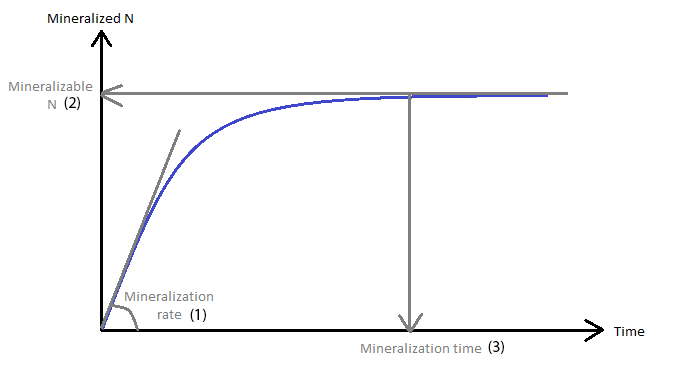
\includegraphics[width=1\linewidth]{intro_Ncum}
	\caption{The nitrogen mineralization curve with its characteristics. The three important characteristics are the mineralization rate at start of the mineralization, the potential mineralizable N and the time to reach the potential mineralizable N}
	\label{fig:intro_Ncum}
\end{figure}

Despite the fact that OM plays an important role in soil fertility and physical structure, OM is not a good indicator for how much N can be mineralized on short term. Changes in OM content take place gradually and subtle, so small changes are difficult to detect \citep{Ghani2002, Hanegraaf2009}. A better indicator would be the labile fractions of the organic pool, such as the easy biodegradable and extractable fractions, as shown in Figure \ref{fig:intro_haynes} \citep{Haynes2005}. Those fractions are measurable parts of organic matter and not the theoretically defined pools of SOM \citep{Wander2004}. Several studies observed significant relationships between EOM fractions and the soil N mineralization \citep{Ros2011a,Ros2012}.  

	\begin{figure}[h]
		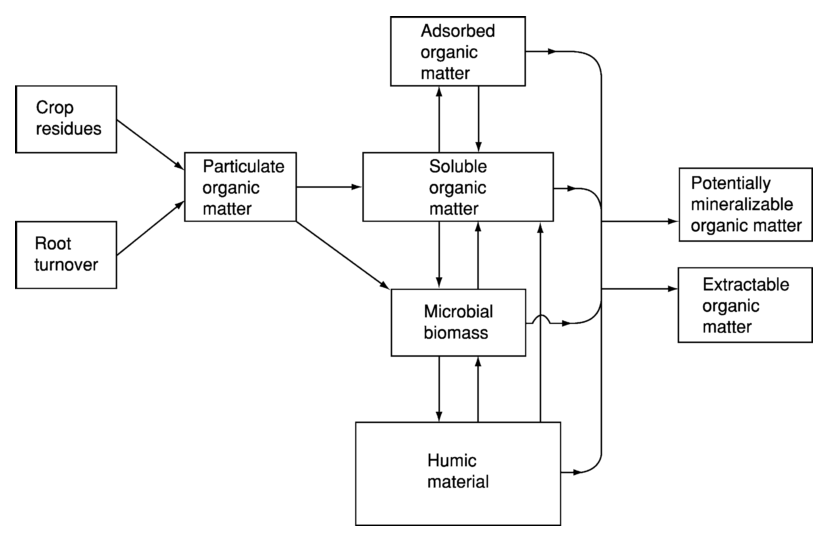
\includegraphics[width=1\linewidth]{intro_haynes}
		\caption{Schematic overview of the relationships between various organic matter fractions. Source: \citet{Haynes2005}.}
		\label{fig:intro_haynes}
	\end{figure}

The classical paradigm is that SOM stability mainly depends on molecular structure of organic material (resistance to breakdown) and humus formation (by condensation reactions). A new view is developing, suggesting that not organic matter quality but other factors strongly determine decomposition \citep{bingham2015}. The resistance to decomposition is regarded as a property which is controlled by environmental factors such as microbial inhibition and distribution and also physical/chemical protection and disconnection \citep{Lutzow2006,Schmidt2011}.


\subsection{Possible indicators for usage in practice}
A soil indicator that can be used in practice for the prediction of N mineralization should met some requirements. \citet{Gil-Sotres2005} appointed the following criteria. The indicator should measure more than only one soil function and should be sensitive to changes in short term. Ideally, reference values  critical values should be known. And last but not least, the implementation of the indicator in practice should be easy, which means it should be simple to analyze with low costs. 

Literature shows that the biological available N pool is related to a.o. the following  measurable indicators that are relevant for practical usage:

\begin{itemize}
	\item \textbf{Hot water extractable carbon (HWC)}. HWC is the organic carbon fraction that is extracted with hot water. The dissolved organic carbon (DOC) fraction, that is initially in the solution, is excluded by first extracting with cold water.  The HWC is strongly related to labile OM and microbial biomass \citep{Ghani2002, Ghani2003}. HWC could possibly be measured with the NIRS methodology (MH), then it could be implemented in routine labs. 
	\item \textbf{Extractable organic nitrogen (EON)}. This is the N part after extraction with for example the hot water extraction. The EON can be an indicator of microbial activity (and so mineralization) though the flow of N through the DON pool controls the rate of mineralization more than its size \citep{Schimel2004}. Big disadvantage of this approach is that EON concentration measurements highly depend on methodology \citep{Ros2009}. 
	
	\item \textbf{Potential nitrogen mineralization (PNM)}. The PNM is an \textbf{aerobic mineralization} analysis method. The PNM is defined as the total mineralized N over 12 weeks or the rate of mineral N production over the 12 weeks (slope of cumulative Nmin curve) of aerobic incubation. Numerous methods have been developed, what is nicely described by a.o. \citet{Doran1996} and \citet{Canali2005}.
	
	\item \textbf{Biological fertility indicator (BFI)}. The BFI is the \textbf{anaerobic mineralization} analysis method. The BFI is defined as the total mineralized N in 7 days under anaerobic conditions.
	
	\item \textbf{Soil respiration (Resp)}. Respiration is probably the process most closely associated with life \citep{Bloem2005}. Soil respiration is measured as \ce{CO2} production and. \ce{CO2} release indicates  that at the same time \ce{O2} is taken up. This occurs when the environment is aerobic.
	
	\item \textbf{Microbial biomass (C-mic)}. Microbial biomass has a high turnover rate, so it is suggested to be a sensitive indicator of changes in tillage systems \citep{Lynch1980, Sparling1997}. It is also related with soil physical characteristics \citep{Schimel1986}. A downside of this indicator is the difficulty of the measurement, but \citet{Sparling1992} suggested HWC and \citet{Myrold1987} suggested the PNM as a good approximation of the microbial biomass. 
	
	\item \textbf{Ratios} such as C/N ratio, fungi/bacteria, HWC/C-total, PNM/C-total, C-mic/C-total. This ratios can be indicators for the stability (degradability) of the organic material in the soil \citep{Sparling1992, Hanegraaf2009} and the intensity the agricultural system \citep{Bloem2004}
	
\end{itemize}
		
	There are various techniques for predicting bioavailable N \citep{Haynes2005}. It can be done by chemical extraction methods or biological incubation methods, but none of these methods is universally accepted \citep{Nannipieri2009}. The mineralization can be simulated in relation to abiotic soil properties or biological indicators. The potential N supply over a period could be predicted by simulation models which are widely available \citep{Manzoni2009}. A nice example is the MINIP model \citep{Janssen1984}, which is used in the Netherlands in several tools for soil management recommendations. Those mineralization models are refined over time for research and for practical usage \citep{Yang2000,Postma2004}.  However, those models are not used in the Netherlands for prediction the mineralization on grassland soils. This is probably because it is difficult to calibrate the models for each specific field due to the heterogeneity of the fields \citep{Ros2015}. 
		
\subsection{Current N recommendations in the Netherlands} % Hanegraaf Zand rapport
Currently, most standard soil management advises for farmers consists of general analyses concerning nutrient amounts in the soil. At present, in the Netherlands, the fertilizer N recommendations fo grasslands are build on the Non Fertilizer N Supply (NFNS, Dutch: NLV), which is based on the work of \citet{Hassink1995a}. The NFNS is defined as the N uptake on unfertilized plots and is calculated by regression models based on the organic N content in the top 0-10 cm soil layer \citep{Bemestingscommissie2012}. The NFNS does not take into account the different degradability of the SOM pools and environmental conditions. The predictions seem not to be accurate for today measurements, as shown for example in Figure \ref{fig:intro_ros}. Deviations from the NFNS predictions are up to 100 kg N per ha, so the farmer does not get fully insight in the potential of the soil to make nutrients free for plant uptake. Hence, it is recommended to upgrade the current fertilizer N recommendations \citep{Hanegraaf2009, VanEekeren2010, Ros2015}. Another issue is that for the fertilizer N recommendations for both grassland and arable soils the same name (NFNS) is used, while different protocols are carried out. For arable soils the recommendations are based on the MINIP model of \citet{Janssen1984} and soil samples are taken from the 0-20 cm soil layer (tilling depth).\\
%review NLV: Bussink 2002
%weer: Ros&Bussink 2012

		\begin{figure}[t]
			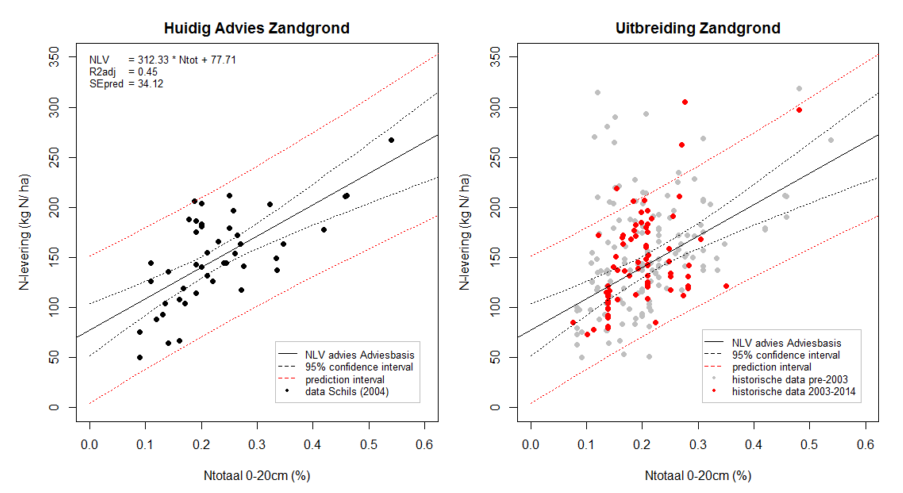
\includegraphics[width=1\linewidth]{intro_ros}
			\caption{Relation between N-total and the predicted N supply (NFNS) in compared with data from experiments on sandy soils. The accuracy of the predictions is currently still too low. Note that the data comes from samples from the 0-20 cm soil layer (normally the samples for grassland soils comes from the 0-10 cm layer.) Source:   \citet{Ros2015}. }
			\label{fig:intro_ros}
		\end{figure}
		
Other countries ....info zoeken over USA, NZ?

  In the ideal situation the farmer knows what amount of N is available for crop growth at each time period, so he can adjust fertilization rates on the grass requirements. Therefore, other variables that influence the N mineralization, such as weather conditions and organic matter quality, should maybe been considered in prediction models \citep{Ros2015}. 

	


	
	
	
	
%%%%%%%%%%%%%%%%%%%%%%%%%%%%%%%%%%%%%%%%%%%%%%%%%%%%%%%%%%%%%%%
\chapter{Materials and methods}
%%%%%%%%%%%%%%%%%%%%%%%%%%%%%%%%%%%%%%%%%%%%%%%%%%%%%%%%%%%%%%%%%%
A existing data set is analyzed for statistical relations between biotic and abiotic soil properties in order to predict soil N mineralization. This relationships were validated with data from field experiments, where grassland soils were analyzed for several key indicators. 

\section{Calibration data: internship Echeverri}
The calibration data is provided by the internship work of  \citet{Echeverri2014}. In his project he tested the following three methodologies to assess SOM quality. 1: Validation of  HWC methodology to predict the biologically decomposable SOM in short term. 2: Understanding SOM pathways by performing incubation and SOM fractionation. 3: Providing insight about thermogravimetric analyses in SOM study.  He suggested that hot water extractable carbon HWC extracted the most labile carbon fraction of soils and therefore he assumed HWC to be an appropriate indicator of SOM decomposability in short term.

For his study Echeverri analyzed 21 soil samples from different agricultural fields in the Netherlands. Soil types differed in SOM and clay content. 
The available data consist of the following analyses. 

	\begin{enumerate}
	\item \textbf{Standard soil parameters} \\
	This data consists of near infra red spectroscopy (NIRS) analyses and classical analyses, both conducted by the lab of \href{http://blgg.agroxpertus.nl/}{\textit{BLGG AgroXpertus}}. This analysis contains about 60 soil parameters that are used in the extensive soil management advices (the BLGG \href{http://blgg.agroxpertus.nl/product/bemesting/bemestingswijzer-bouwland}{\textit{'Bemestingswijzer'}}). 
	
	\item \textbf{Mineralization indicators}\\
	Soil life indicators are used to give a measure of the activity of the soil live. Microbial activity is often linked to the potential quantity of N that can be mineralized. 
	\begin{itemize}
		\item The potential nitrogen mineralization (PNM).  Units: mg N kg $^{-1}$ per day. The data of \citep{Echeverri2014} shows only significant values for \ce{NO3}, because all concentrations of \ce{NH4} were below the detection limit. 
		\item The biological fertility indicator (BFI). Units: mg N kg $^{-1}$. Measurements were done on field wet soils (BFI-w) and on dried soils (BFI-d). 
	\end{itemize}
	
	\item \textbf{HWC} \\
	HWC is calculated as the difference between the inorganic and organic carbon after hot water extraction. Units: mg C kg $^{-1}$.   
	
	\item \textbf{Potential soil respiration rate (Resp)}\\
	The soil microbe respiration is measured as \ce{CO2} production at optimum moisture and temperature. Units: mg C kg $^{-1}$.   
	%add some more information
\end{enumerate}

All data of Echeverris study can be found in Appendix \autoref{chap: Calibration data}. This data is used for calibrating the statistical models for predicting N mineralization.  

Possible indicators for the prediction of N mineralization that are measured for the calibration data are the PNM, HWC, Resp and the BFI. The opportunity for introduction of mineralization indicators in practice depends on the accuracy and precision of the measurements and how easy it is to automate the analysis of the indicator to make routine determinations more efficient. Hence, both HWC and BFI seems to have the most positive perspectives to be implemented into fertilization advisement tools, because the possibility to measure these indicators with the NIRS method \citep{Hanegraaf2008, Vasques2009}. 

% A short study is conducted on the performance of different BFI methodologies (Appendix \ref*{chap:bfis}). 


\section{Validation data: grassland soils Friesland}
The statistical models are validated with data that is collected from dairy farms that also join the NMI project "Verborgen rendement uit de bodem". Within the scope of this project it was only possible to analyze the soil for HWC and PNM as indicators for the N mineralization. 

All validation data can be found in Appendix \autoref{chap: Validation data}.

\subsection{Field selection and sampling}
Soils were collected from grassland soils at four dairy farms in Friesland. The chosen fields are also used for other research of NMI on the dynamic spatial and temporal nitrogen behavior. All fields ranged from 2.5-5.3 ha and consists of sandy soils, with some loamy characteristics. %misschien meer over zeggen? 

\begin{table}[ht] %Table Field information
	\caption{Field information and soil characteristics of the top layer (0-10 cm) for the growing season of 2015 (Sampling on 06/16/2015) }
	\footnotesize 
	\renewcommand{\arraystretch}{1.2}
	
	
	\begin{tabu} to \textwidth{@{}X[c]X[l]X[l]X[c]X[l]X[l]X[l]@{}}% {@{}rrrrrrr@{}} 
		\toprule	\rowfont{\bfseries}
		Farm & Place & Location & OM (\%) & Clay (\%) & Ntot (mg/kg) & pH \\  \midrule
		A & Olderbekoop & Lat: 52.94 Lon: 6.13 & 8.4 & 3 & 3990& 5.6 \\
		B & Olderbekoop& Lat: 52.93 Lon:6.11 & 4.5& 2& 1670& 5.8\\
		C & Nijeberkoop & Lat: 52.96 Lon: 6.19 & 6.8& $<$1& 2820& 5.9\\
		D & Appelscha & Lat: 52.96 Lon: 6.42 & 7.3& 2& 2890& 5.6\\		 \bottomrule
	\end{tabu}
	
\end{table}

Each grassland field was harvested several cycles and was alternately cut for silage and grazed. The initial protocol was that within a week before each cutting upward of the second cutting, we should have taken a sample of the fields \ref{fig:mm_samples} and subsequently analyze the samples for the indicators. Having regard to the diversity in farming methods and difference in cutting times, we toke samples at fixed dates.  Even when grazing was applied, a sample was taken at the same time as it was done from the other fields. Samples were taken on 06/16/2015, 07/03/2015, 03/08/2015 and 04/09/2015. All samples were taken from the 0-10 cm top soil layer of each field. Per sample, $>$70 subsamples were taken in W-pattern. To show the heterogeneity of the soils, on 07/03/2015 different samples were taken from characteristic field areas for each farm (Appendix \ref{chap: study1}).

\begin{figure}[h] %Figure Sampling Time Plan
	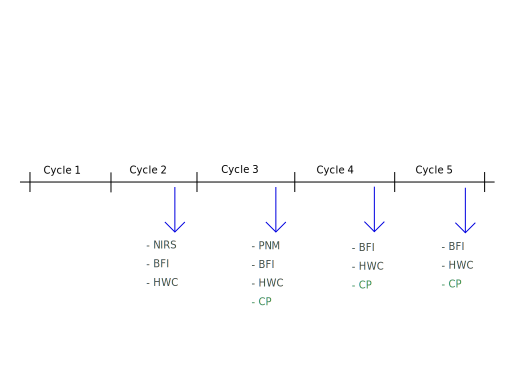
\includegraphics[width=1\linewidth]{mm_samples}
	\caption{Sample time plan of the Friesland samples. The first cycle was missed. From the second to the last cycle, the BFI and the HWC was measured. For the second cycle, the NIRS analyses was done. For the third cycle, the samples for the PNM analysis were taken. From the third to the last cycle, the herbage indicators were determined (relevant: crude protein (CP). Ideally, all samples has to be taken within the same timespan before the grass cutting and without fertilization and manure application. However, this was not feasible within the project, because it was not communicated with the farmers beforehand.}
	\label{fig:mm_samples}
\end{figure}

\subsection{Soil analysis methods}
Soil samples were mixed by hand and passed through a 5-mm sieve. Big roots and grass leafs are removed. The samples were stored field-moist at a temperature of 4 °C. Analysing methods are done within 10 days after sampling. 
The complete protocols used for the chemical and physical analysis are described in Appendix \ref{chap: Protocols}. In short the following procedures were done. 

\subsubsection{How water extractable carbon}
The HWC was determined according to the method used by \citet{Ghani2003}. First 30 ml of distilled water was added to  3 g of dried soil. The tubes were shaken in a vortex shaker during 30 min, centrifuged at 3600 rpm during 20 min. Subsequently, 30 ml of water was added to the settlement. The tubes were shaken 30 min and next were placed in a stove at 80 ˚C during 16 hours. Afterwards, the tubes were centrifuged at 3600 rpm during 20 min. Finally, the supernatant were filtered using a 0.45 µm filter and the DOC was analyzed using a TOC analyzer. 

\subsubsection{Aerobic nitrogen mineralization}
The PNM was determined according to the protocol described by \citet{Ros2014}. Sample moister contents were set to about 60\% of the water holding capacity (WHC). The WHC was determined by the addition of water to dried soil until it became saturated and a water film was growing on the surface. Subsequently, 100 g of the homogenized sample was put in polyethylene bags that were permeable for \ce{CO2} and \ce{O2} , but not for \ce{H2O} molecules. After sealing the samples were set in a room at constant temperature of 20°C. Samples were analyzed for mineral N by the BLGG lab after 1, 3, 6, 9 and 12 weeks. 

\subsubsection{BFI}
The anaerobic mineralization incubation was conducted by the BLGG lab. The lab followed the procedure of (aan Richard vragen, 7 days anareobic incubation)
%zie book 



\section{Statistical analysis}
Data were analyzed with R (v. 3.1.3), using the RStudio IDE and a.o. the packages pls and lm. 
\subsection{Calibration}
Three data points were removed because they contained erroneous data (PNM was close to 0 or $<$ 0, see Appendix \ref{chap: Calibration data}). For the PNM, only validation data of \ce{NO3} is used, because accurate \ce{NH4} data were not available for the calibration data. 

All data of one parameter set are log transformed when necessary to met the normality requirements (test of \citet{Shapiro1965}). Parameter sets were not normally distributed when grouping them into soil types. Data of the classical soil analysis is used, because the NIRS analysis are based on the classical analyses. When data of the classical soil analysis was not available, data of the NIRS analysis was used. This was not completely possible for the organic carbon measurements, because not all data was available for both the classical and the NIRS analysis. 
Partial least squares (PLS, \citep{Mevik2013}) regression was applied on the transformed data to get insight in the variation of the modeling approaches and to select the relevant parameters. 
Several models were made to predict the N mineralization on grassland soils. To get a first insight in the relative importance of the variables, a stepwise regression was carried out which was based on the Akaike information criterion (AIC, \citep{Sakamoto1986}). Multi-linear models with interaction terms were made by trial and error. 

\subsection{Validation}
The models are validated with the Friesland soil samples. All data is evaluated to see how large the difference is between the observed values and the predicted values. For evaluating the validity of the models we use the coefficient of variation and the analysis of residuals. 






%%%%%%%%%%%%%%%%%%%%%%%%%%%%%%%%%%%%%%%%%%%%%%%%%%%%%%%%%%%%
\chapter{Results}
%%%%%%%%%%%%%%%%%%%%%%%%%%%%%%%%%%%%%%%%%%%%%%%%%%%%%%%%%%%%
The results shows that the N mineralization could be predicted by some simple and multivariate linear models. However, 
%-----------------------------------------------------------------------------------------------------------------------------------------------------------
\section{Calibration}
%-----------------------------------------------------------------------------------------------------------------------------------------------------------
\subsection{Soil properties}
The soils of the calibration set are collected from agricultural fields from over the Netherlands. The 21 soils consists of different clayey, sandy and peaty soils. Hence, they varied widely in their physical and chemical characteristics (Table \ref{tab: resuls_char}). The key factors varied between 17 and 71 mg N kg $^{-1}$ for the PNM rate and between 239-5099 mg C kg $^{-1}$ for HWC. 

	\begin{table}[h] % Tabel met overzicht van alle bodem variables
	\caption{Relevant variables that were used for the data analysis (\textit{n=18}). Data from internship \cite{Echeverri2014}. Outliers with incorrect data were removed (\textit{n=4}).}
	\footnotesize 
	\renewcommand{\arraystretch}{1.2}
			\begin{tabu} to \textwidth{X[1.5,l]X[1.5,l]X[1,r]X[1,r]X[1,r]X[1,r]X[1,r]}
			\toprule \rowfont{\bfseries}
			& Units & Mean & Median & SD & Min & Max \\ \midrule \rowfont{\bfseries}
		Mineralizable N & mg N kg$ ^{-1} $ & 35 & 26 & 18 & 14 & 71 \\  
		HWC & mg C kg$ ^{-1} $ & 1231& 877 & 1191 & 239 & 5099 \\ 
		Total N & g N kg$ ^{-1} $ & 2.79 & 1.77 & 2.33 & 0.95 & 9.38 \\ 
		Total C & g C kg$ ^{-1} $ & 3.78 & 2.30 & 3.26 & 0.90 & 10.70 \\ 
		BFI & mg N kg$ ^{-1} $ & 70 & 47 & 58 & 16 & 248 \\ 
		Respiration & mg C kg$ ^{-1} $  & 11.8 & 7.7 & 12.2 & 3.0 & 55.3 \\ 
		OM & \% & 7.8 & 4.8 & 5.9 & 2.4 & 20.2 \\ 
		Organic C & \% & 2.39 & 2.10 & 1.45 & 0.90 & 6.10 \\ 
		Initial moisture & g \ce{H2O} g$ ^{-1}$ & 1.88 & 1.50 & 1.18 & 0.60 & 4.60 \\ 
		C:N ratio & -  & 12 & 10 & 4 & 8 & 20 \\ 
		\ce{NO3} & mg N kg$ ^{-1} $ & 32.6 & 26.4 & 24.1 & 4.4 & 87.1 \\ 
		\ce{NH4} & mg N kg$ ^{-1} $ & 4.8 & 3.7 & 4.2 & 1.4 & 18.9 \\ 	
		pH & - & 6.1 & 6.4 & 0.9 & 4.6 & 7.2 \\ 
		\ce{CaCO3} & \% & 1.7 & 0.2 & 2.8 & 0.2 & 11.4 \\ 
		CEC & mmol+ kg$ ^{-1} $ & 166 & 120 & 115 & 53 & 447 \\ 
		Silt & \% & 24.5 & 24.0 & 17.2 & 5.0 & 63.0 \\ 
		Sand & \% & 54.2 & 50.0 & 29.0 & 2.0 & 90.0 \\ 
 			 \bottomrule
			
	\end{tabu}
	\label{tab: resuls_char}
\end{table}

	\begin{figure}[ht] % boxplots van bodemeigenschappen
		
		\centering
		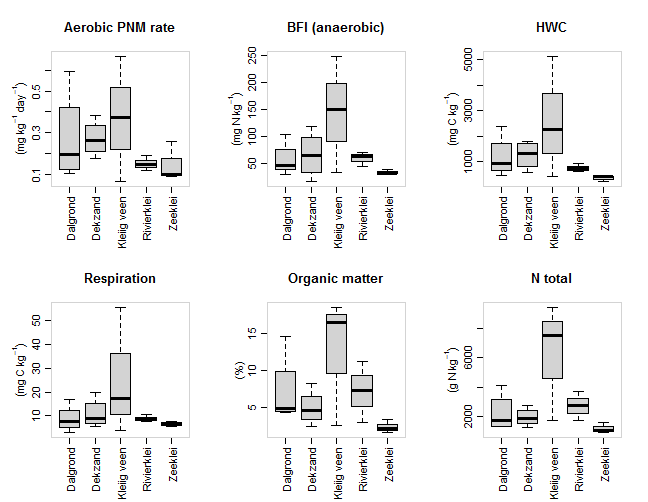
\includegraphics[width=1\linewidth]{results_boxplots}
		\caption{Boxplots of key soil mineralization indicators grouped on soil type: dalgrond (\textit{n=4}), dekzand (\textit{n=4}), kleiig veen (\textit{n=3}), river clay (\textit{n=3}) and sea clay (\textit{n=3}). It shows  that much of the variation could be explained by soil type}
		\label{fig:results_boxplots}
	\end{figure}
Figure \ref{fig:results_boxplots} shows the variability of the key indicators for soil N mineralization. Much of the variation could be explained by the differences in soil types. This shows the disadvantage of combining all data. However, because the small dataset, we will merge all soil types for the statistical analysis.

\subsection{Soil indicators for N mineralization} 
In this study there are four different biological essays on the N supply that can be used as indicator for the N mineralization. They consists of the aerobic longterm measurements on dried soils (PNM), the anaerobic measurements on dried soils (BFI-d), the anaerobic measurements on moist soils (BFI-w) and the NIRS measurement of the BFI-w (BFI-nir). We assume the aerobic PNM the best predictor of the real mineralization, because it approximates the field conditions the most. Hence, the PNM is used as response variable. 

 \subsubsection{Aerobic mineralization rate as response variable} 
During the 12 weeks aerobic mineralization, the cumulative mineral N (here \ce{NO3}) increased on average up to 35 mg kg$^{-1}$ for all soils (Figure \ref{fig:results_Ncum}). Cumulative mineralization was the highest for peaty soils (47 mg kg$^{-1}$) and the lowest for clayey soils (24 mg kg$^{-1}$).  In the 12 weeks incubation period, we assume the N mineralization to be still in the linear phase (see Figure \ref{fig:intro_Ncum}). Subsequently, we consider the slope of the cumulative N mineralization curve as an indicator for the N mineralization. The mean mineralization rate  is 0.19 mg N kg$^{-1}$ per day. Soil type had a strong effect on the mineralization rate: for sandy soils the average mineralization rate was 0.26 mg N kg$^{-1}$, for clay soils 0.14 mg N kg$^{-1}$  and for the peaty soils 0.34 mg N kg$^{-1}$. The variance was greatest for the sandy and lowest for the clayey soils. 
	\begin{figure}[h] % Plotje van cumulative N min. Friesland data nog toevoegen.
	\centering
	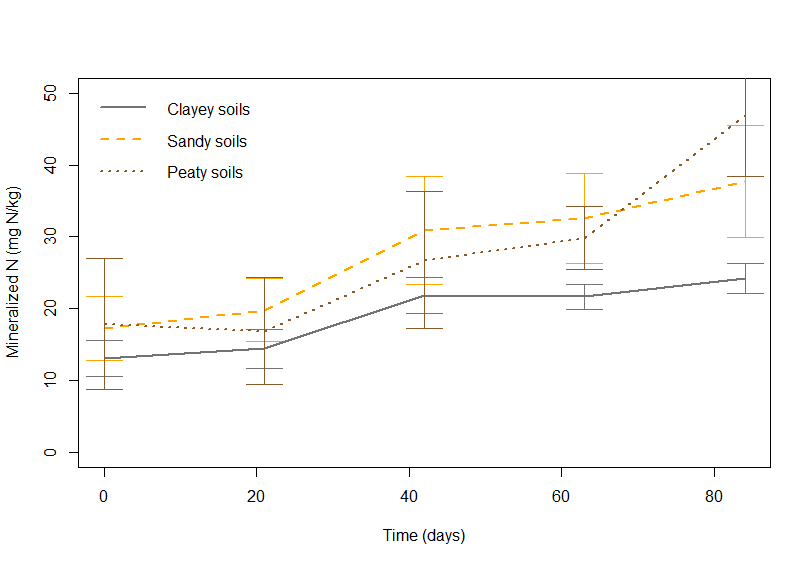
\includegraphics[width=0.8\linewidth]{results_Ncum}
	\caption{Cumulative aerobic N mineralization over time for the different soil types. Error bars denotes the standard error of the means. The mean mineralization rate (slope) of all soils is 0.19 mg N kg$^{-1}$ per day}
	\label{fig:results_Ncum}
\end{figure}

Soil indicators shows various correlations (Figure \ref{fig:results_corr}), despite of the high variation in soil characteristics (\ref{tab: resuls_char}). As expected, in particular the indicators for labile organic matter shows good correlation with the aerobic mineralization. 
	\begin{figure}[h] %Correlatie matrix
	\centering
	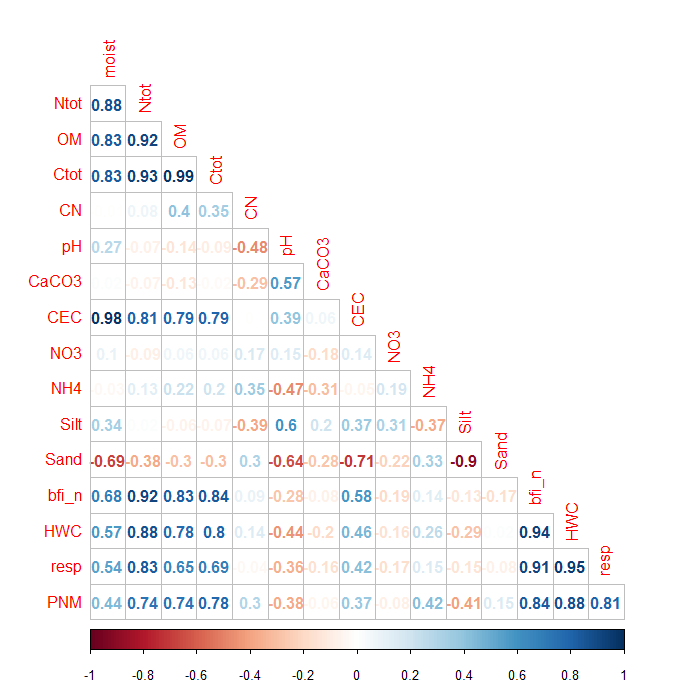
\includegraphics[width=0.7\linewidth]{results_corr}
	\caption{Correlation matrix. Red numbers denote negative and blue positive correlations. Lower color intensity indicates less correlation.}
	\label{fig:results_corr}
\end{figure}

The variability of the potential mineralization rate (mg N kg$^{-1} $ day$^{-1}$ ) is mainly explained by a component that is related to organic matter. This is shown in the PLS output in Figure \ref{fig:results_pls}. Highest related indicators were HWC, respiration, C/N ratio, BFI, pH, Silt and CEC. This component explains about 37\% of the variability when outliers were removed. The second explanatory component is probably related to more chemical-physical properties of the soils, though this were weak relationships and it only explains 13\% of the variability. However, when applying PLS analysis with the BFI as response factor, it becomes more clear that textural characteristics also have a (minor) influence on the response. 
	\begin{figure}[ht] % Plotje PLS output.
	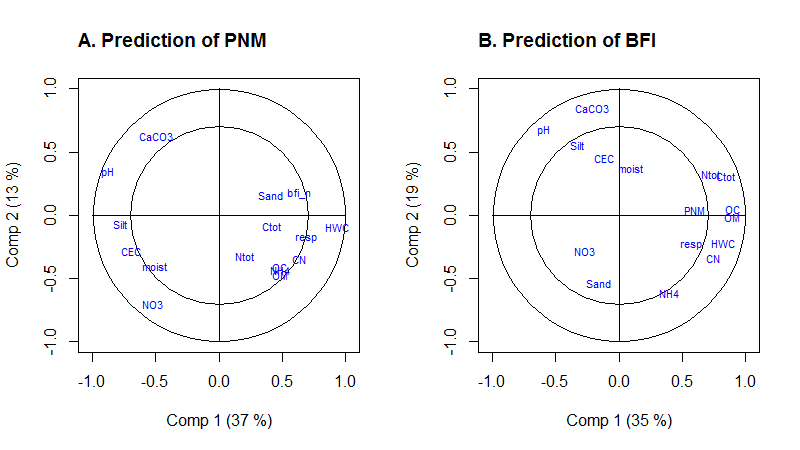
\includegraphics[width=1\linewidth]{results_pls_pnmbfi}
	\caption{PLS output of all variables with potential N mineralization rate as response variable. \textbf{A.} PLS regression for the prediction of PNM. The first component explained 37\% of the variance and the second component 13\%. \textbf{B.} PLS regression for the prediction of BFI. The first component explained 35\% of the variance and the second component 19\%. It is clear from both pictures that the most of the variance is explained by the component that is related to organic matter.}
	\label{fig:results_pls}
\end{figure}


\subsubsection{Descriptive models for prediction of N mineralization}
As shown in Figure \ref{fig:results_models}, PNM was significant related to the indicators for labile organic matter: HWC (R$^{2}$=0.7, \textit{p} $<$0.001), Resp (R$^{2}$=0.6, \textit{p} $<$0.01) and BFI (R$^{2}$=0.6, \textit{p} $<$0.01). The direct relationship with OM was relatively poor (R$^{2}$=0.4, \textit{p} $<$0.01).

\begin{figure}[ht] % Plotje van 6 lineaire modellen
	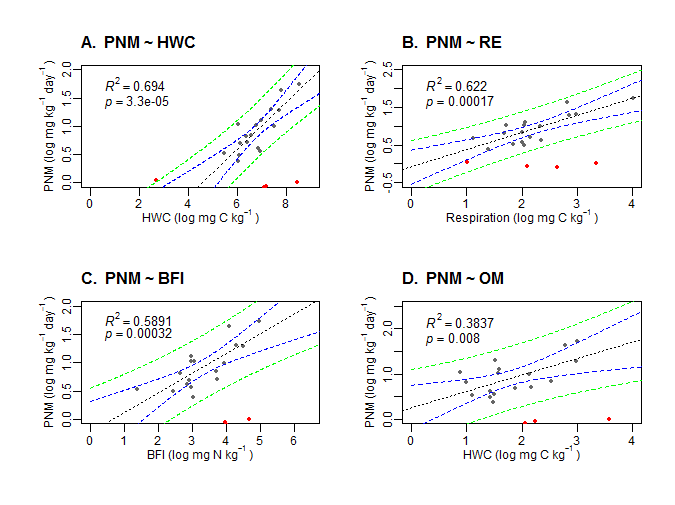
\includegraphics[width=1\linewidth]{results_models}
	\caption{Linear relationships with potential N mineralization rate (mg N kg$^{-1}$ day$^{-1}$). Blue lines indicate the prediction intervals, green lines indicate the confidence intervals and the red dots are the outliers values. Note that all plots are from models with an intercept term.}
	\label{fig:results_models}
\end{figure}

Significant (\textit{p}$<$0.001) models for the prediction of N mineralization were obtained from the calibration dataset (\ref{tab: resuls_mods}).
 Here we played around with removing and adding intercept and interaction terms. 
 It turns out that addition of Resp in the multivariate approach ends up in more significant models. This is what we expected, because the single relation of Resp with PNM was relatively high compared with the other variables. 
 The best model with Resp was the one with an interaction term between C total and sand. However, the only suggestive explanation could be the fewer protection of SOM by the sand.  We can not explain this interaction clearly, so we reject the validity of this model. 
 
 The second best model with Resp was the one with an interaction term between C total and C/N ratio. This seems more logical, because this considers the relative value of total C in the soil which is interacting with the C/N ratio (stability of the SOM). However, when only adding the C/N ratio, the model was not significant, what is contradictory with the model. 
 
 The second best model we identified was the model were HWC is interacting with OM, what is an understandable interaction.  Because the HWC is expected to be measured with the NIRS method in future \citep{Vasques2009} and respiration is quite difficult to analyze, we choose the last model. With the parameter estimates this model is: 
\begin{equation} %choossen model
PNM rate = 0.13\cdot HWC -1.05\cdot OM +0.15\cdot HWC:OM
\label{eq: model}
\end{equation}
Specific statistical characteristics of this model can be found in \ref{tab: resuls_mods}. Note that this relationship should be applied to the log transformed values of PNM, HWC and OM. 

\begin{table}[hb] % Table model output
		\caption{Model output for the prediction of PNM. For the models,  '-1' denotes the absence of an intercept in the model,  ':' an interaction term without single variables included and '*' an interaction term plus both single variables included in the model. Prediction variables are m (moister content), om (OM content), ct (C-total), cn (C/N ratio), no (\ce{NO3}), nh (\ce{NH4}), sa (sand), bf (BFI), hw (HWC), re (respiration)}
		\footnotesize 
		\renewcommand{\arraystretch}{1.2}
		
		\begin{tabu} to \textwidth{X[1,l]X[3,l]X[1,r]X[1,r]X[1,r]X[1,r]X[1,r]X[1,r]}
			\toprule \rowfont{\bfseries}
 & Model & R$^2$adj & AIC & BIC & RSS & SE-pred & pval \\ 
 \midrule
&\textit{Simple Linear models}& & & & & & \\
1 & hw & 0.67 & 1.5 & 4 & 0.76 & 1.25 & 3.3e-05 \\ 
2 & re-1 & 0.94 & 3.27 & 4.94 & 0.95 & 1.28 & 2e-11 \\ 
3 & bf-1 & 0.93 & 5.43 & 7.09 & 1.08 & 1.3 & 5.5e-11 \\ 
4 & ct-1 & 0.83 & 21.38 & 23.05 & 2.77 & 1.52 & 1.1e-07 \\ 
5 & nt-1 & 0.88 & 15.45 & 17.12 & 1.95 & 1.42 & 6.3e-09 \\ 
6 & om-1 & 0.89 & 13.81 & 15.48 & 1.77 & 1.39 & 2.9e-09 \\   \addlinespace[0.5cm]
&\textit{Mixed linear models}& & & & & & \\
 7 & hw+hw:ct-1 & 0.94 & 3.11 & 5.6 & 0.84 & 1.27 & 1.6e-10 \\ 
 8 & hw*om-1 & 0.95 & 0.63 & 3.96 & 0.65 & 1.24 & 3.5e-10 \\ 
 9 & hw+ct+nt & 0.67 & 3.33 & 7.5 & 0.67 & 1.26 & 0.00053 \\ 
 10 & hw+hw:om+om:ct & 0.72 & 0.46 & 4.62 & 0.57 & 1.23 & 0.00018 \\ 
 11 & re+nh+no-1 & 0.95 & 1.82 & 5.15 & 0.69 & 1.25 & 5.7e-10 \\ 
 12 & re+cn:ct-1 & 0.95 & 0.32 & 2.82 & 0.71 & 1.24 & 4.7e-11 \\ 
 13 & re+ct:sa-1 & 0.96 & -3.92 & -1.42 & 0.56 & 1.21 & 7.2e-12 \\ 
 14 & om+om:bf & 0.61 & 5.43 & 8.76 & 0.86 & 1.28 & 0.00056 \\
\bottomrule
			
		\end{tabu}
		\label{tab: resuls_mods}
	\end{table}


%-----------------------------------------------------------------------------------------------------------------------------------------------------------
\section{Validation}
%-------------------------------------------------------------------------------------------------------------------------------------------------------
Insert Table validation data and give comments.
	\begin{figure}[ht] % boxplots soil indicators per Farm
		\centering
		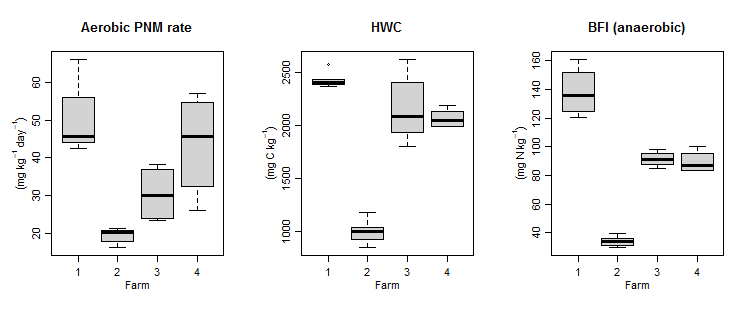
\includegraphics[width=1\linewidth]{results_valbox}
		\caption{Boxplots of validation data of the key soil mineralization indicators per farm.}
		\label{fig:results_valbox}
	\end{figure}

The model to predict the aerobic PNM rate (\ref{eq: model}) overestimates the real measurements (Figure \ref{fig:results_pm}). In addition, the linear relationship plots (Figure \ref{fig:results_models}) shows that ... \textbf{wachten op data}  

	\begin{figure}[ht] % predicted vs observed values van model PNM = 0.13HWC -1.05 OM +0.15 HWC:OM
		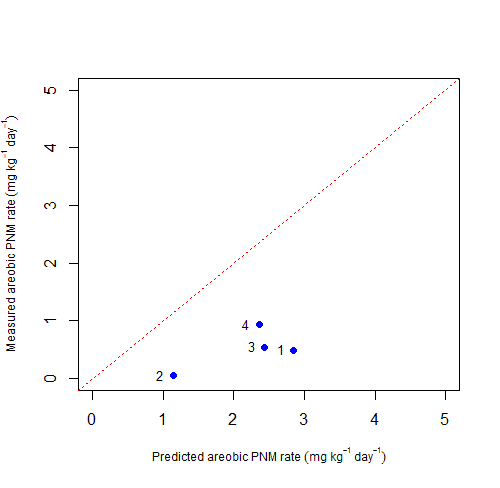
\includegraphics[width=0.7\linewidth]{results_pm}
		\caption{Predicted vs. measured values of the aerobic PNM rate. Prediction is based on model \ref{eq: model}}
		\label{fig:results_pm}
	\end{figure}
	

	
	
	


\chapter{Discussion}
% slope of Nmin cum as indicator for PNM: \cite{Hassink1994}
% already noted by Ros2011 that a direct predictor of the N uptake based on soil indicators not possible
   \section{General remarks}
   \subsection{Limited statistical power}
   The used dataset of \citet{Echeverri2014} was limited for several reasons. It was possible to identify some relationships, however the question arises how meaningful this relationships are. The following issues causes the naughty statistical analysis. 
		   \begin{itemize}
   	\item The limited size of the dataset. Only 21 soils were measured.  Given the wide range in soil characteristic values, this is way to little to identify solid relationships.
   	\item The unreliability of the data. Four outliers were excluded, because they contained erroneous data. This is almost 20\% of the total dataset, so
   	 the reliability of the remaining data is debatable too . 
   	\item The heterogeneity of the soils. The samples were from different soil type and differed huge in e.g. OM- and clay content. Much of the variation could be explained by the differences in soil types (Figure \ref{fig:results_boxplots}). This shows the need for studying relationships per soil type. 
    \end{itemize} 
   
   Additionally, the validation dataset had also some problems that influences the results. The following troubles appeared during the project.
		   \begin{itemize}
	\item Samples were taken from the 10 cm top soil layer, whereas the calibration data says that the samples from \citet{Echeverri2014} were taken from the 25 cm top soil layer. Soil characteristics certainly differ for both soil layers, but the consequences for the statistical relations were not identified. 
   	\item Soils were manured several times during the growing season, which could have influenced the outcomes of the soil analyses. 
   	\item The soil heterogeneity within the fields was notable, which is shown in Appendix \ref{chap: study1}. Despite the fact that a proper sampling strategy was applied ($>$70 subsamples taken in W-pattern), sample differences could be considerably. 
   \end{itemize}
   
   I did the statistical analysis despite the limitations of the available data. For my internship project it was especially important to formulate the general pattern of identifying relationships for the prediction of N mineralization by doing applied research. 
   
	\subsection{Applicability of relevant indicators}
	\subsection{Relation between aerobic mineralization and HWC}

	\section{Prediction of N mineralization}
	The choossen model 

	
	\subsection{Explaining the variability}
	\subsubsection{This study}
	\subsubsection{Environmental factors}
	
	\section{Influence of other factors}
	\subsection{Soil biology}
	We know that mineralization capacity (potential mineralization amount) and -rate depends on the mineralization microbes 
	\subsection{Ratios between soil chemical elements}
	The N mineralization could also be influenced by other soil chemical factors. 
	\subsection{Corrections for environmental influences}
	As already mentioned in the state of the art (Chapter \ref{chap: state of the art}), the variation of N mineralization is not only caused by soil characteristics, but also for a great extend by environmental factors. Temperature and moisture status has high influence on the activity of microbes (ref)


	
\chapter{Recommendations}
	\section{Linking N mineralization to forage quality}
Until now we focused on the linkage between soil indicators and N mineralization. The next step is to relate the N mineralization to grass production in terms of forage quality. A possible indicators is the crude protein, which indicates how much 

	 \section{Statistical methods}
	 \subsection{Data}
Furthermore, I recommend to apply multivariate statistics on large datasets. Those datasets could also consist of measurements from the past. For example, the NMI is already applying research for more than 50 years. Within this time a huge amount of data is gathered. It would be great if this data could be analyzed to identify relationships between soil indicators, N mineralization and forage quality. 
	\subsection{Statistical techniques}
	Multivariate statistical methods that can be use to analyze huge datasets for relevant significant relations are for example ...
	
	\section{Practical tools}
	Farmers wish straightforward tools that can be implemented in their soil nutrient management planning schemes. In future it is maybe possible to develop a self learning fertilization advice tool which take into account the soil history for each field and the weather forecast of the near future. With the knowledge we have until now it is also possible to construct
	




\footnotesize 
\bibliographystyle{abbrvnat}
\bibliography {library}
\normalsize 




\begin{appendices}
	


\chapter{Calibration data}
	\label{chap: Calibration data}
	%Omschrijven waarom ourliers weggelaten moeten worden. 
	
		\begin{table}[ht] % Tabel met overzicht van alle bodem variables
			\caption{Soil parameters that were used for the data analysis. Data from internship \cite{Echeverri2014}.}
			\tiny 
			\renewcommand{\arraystretch}{1.2}
			
			\begin{tabu} to \textwidth{X[2,l]X[l]X[l]X[l]X[l]X[l]X[l]X[l]X[l]X[l]X[l]X[l]X[l]X[l]X[l]X[l]X[l]X[l]X[l]X[l]X[l]X[l]}
				\toprule \rowfont{\bfseries}
 & 1 & 2 & 3 & 4 & 5 & 6 & 7 & 8 & 9 & 10 & 11 & 12 & 13 & 14 & 15 & 16 & 17 & 18 & 19 & 20 & 21 \\ \midrule

db.klas.Vocht & 0.5 & 0.6 & 0.9 & 0.9 & 2.4 & 4.5 & 1.3 & 2.3 & 3.0 & 2.6 & 1.7 & 1.5 & 2.8 & 2.8 & 0.8 & 1.9 & 4.6 & 4.1 & 0.9 & 0.9 & 1.3 \\ 
db.klas.N\_tot & 200.0 & 1290.0 & 1330.0 & 1340.0 & 4150.0 & 5850.0 & 1740.0 & 2780.0 & 3690.0 & 2960.0 & 1590.0 & 1090.0 & 2190.0 & 4200.0 & 950.0 & 1750.0 & 7510.0 & 9380.0 & 1770.0 & 2050.0 & 2760.0 \\ 
db.klas.OS & 0.5 & 2.7 & 4.8 & 4.5 & 16.1 & 35.7 & 4.2 & 8.8 & 12.5 & 7.8 & 4.2 & 3.0 & 6.5 & 9.4 & 2.4 & 4.4 & 19.9 & 20.2 & 4.9 & 4.6 & 8.5 \\ 
db.klas.C\_org & 0.1 & 1.3 & 2.7 & 2.1 &  &  & 1.5 & 3.8 & 6.1 & 2.7 & 1.6 & 1.0 & 2.1 & 3.8 & 0.9 & 1.4 &  &  & 2.5 & 2.1 & 4.3 \\ 
db.klas.C\_tot & 0.4 & 1.2 & 2.5 & 2.3 & 9.0 & 15.1 & 1.4 & 3.7 & 6.1 & 2.4 & 1.5 & 0.9 & 2.3 & 3.7 & 2.0 & 1.7 & 10.7 & 10.5 & 2.3 & 2.0 & 4.1 \\ 
db.klas.CN & 5.0 & 10.1 & 20.3 & 15.7 &  &  & 8.6 & 13.7 & 16.5 & 9.1 & 10.1 & 9.2 & 9.6 & 9.0 & 9.5 & 8.0 &  &  & 14.1 & 10.2 & 15.6 \\ 
db.nir.pH & 7.6 & 7.0 & 5.0 & 5.0 & 5.6 & 4.5 & 5.7 & 6.8 & 6.8 & 5.7 & 6.5 & 6.4 & 7.2 & 6.9 & 7.2 & 7.1 & 6.8 & 5.3 & 5.1 & 5.0 & 4.6 \\ 
db.nir.KZK & 6.1 & 0.8 & 0.2 & 0.2 & 0.2 & 0.2 & 0.2 & 1.7 & 2.7 & 0.2 & 0.2 & 0.2 & 2.0 & 0.5 & 11.4 & 4.0 & 2.7 & 1.0 & 0.2 & 0.2 & 0.2 \\ 
db.nir.CEC & 11.0 & 75.0 & 71.0 & 76.0 & 236.0 & 328.0 & 110.0 & 216.0 & 285.0 & 220.0 & 146.0 & 120.0 & 282.0 & 287.0 & 73.0 & 172.0 & 447.0 & 331.0 & 69.0 & 53.0 & 68.0 \\ 
db.nir.Bodemleven & 1.0 & 16.0 & 29.0 & 47.0 & 103.0 & 137.0 & 62.0 & 44.0 & 69.0 & 85.0 & 31.0 & 30.0 & 46.0 & 80.0 & 38.0 & 32.0 & 150.0 & 248.0 & 50.0 & 118.0 & 79.0 \\ 
db.nir.NO3 & 1.2 & 9.5 & 18.0 & 41.2 & 87.1 & 32.7 & 26.4 & 48.6 & 41.0 & 7.8 & 43.0 & 59.4 & 17.0 & 47.4 & 5.5 & 73.6 & 19.1 & 14.6 & 32.6 & 13.7 & 4.4 \\ 
db.nir.NH4 & 1.2 & 1.5 & 4.9 & 3.3 & 10.1 & 9.1 & 3.7 & 3.1 & 2.5 & 1.5 & 1.7 & 4.2 & 2.8 & 2.3 & 1.4 & 2.9 & 5.4 & 5.5 & 18.9 & 5.5 & 3.9 \\ 
db.nir.Silt & 0.0 & 8.0 & 5.0 & 6.0 & 11.0 & 4.0 & 47.0 & 63.0 & 43.0 & 36.0 & 32.0 & 35.0 & 33.0 & 31.0 & 24.0 & 39.0 & 24.0 & 21.0 & 8.0 & 9.0 & 8.0 \\ 
db.nir.Zand & 92.0 & 87.0 & 90.0 & 85.0 & 73.0 & 69.0 & 38.0 & 2.0 & 11.0 & 25.0 & 50.0 & 49.0 & 32.0 & 34.0 & 56.0 & 34.0 & 23.0 & 38.0 & 85.0 & 85.0 & 83.0 \\ 
db.hwc.HWEC & 15.0 & 576.0 & 877.0 & 1015.0 & 2389.0 & 4660.0 & 933.0 & 609.0 & 725.0 & 1195.0 & 446.0 & 239.0 & 452.0 & 1293.0 & 416.0 & 423.0 & 2262.0 & 5099.0 & 1054.0 & 1625.0 & 1796.0 \\ 
db.hwc.Resp\_mg.kgsoil.day & 2.7 & 5.4 & 7.7 & 7.4 & 16.9 & 28.1 & 10.5 & 8.5 & 7.5 & 14.1 & 7.7 & 6.3 & 3.0 & 8.1 & 5.5 & 4.0 & 17.4 & 55.3 & 7.8 & 19.8 & 10.3 \\ 
db.pnm.X12 & 1.1 & 22.7 & 29.8 & 21.6 & 70.8 & 0.6 & 16.8 & 25.5 & 23.4 & 11.0 & 21.7 & 32.0 & 13.7 & 12.0 & 26.0 & 39.1 & 37.8 & 63.7 & 66.4 & 51.3 & 25.4 \\ 
				\bottomrule
				
			\end{tabu}
			
		\end{table}




\chapter{Validation data}
		\label{chap: Validation data}
		

\chapter{Analysis protocols}
		\label{chap: Protocols}
\chapter{Small study 1: on Farm nutrient management}
		\label{chap: study1}
		The relations between soil quality and forage production and farm management were evaluated. 
			\section{Whole farm soil characteristics}
	We made an overview of the soil characteristics of all fields of the farms. Long term (25 y) data from the farms were provided by the farmers. All routine lab analysis reports were merged to show some trends in  soil fertility of the farms. For the fields on which we took the validation samples, we also studied the heterogeneity of the fields to emphasize the difficulty and pitfalls of soil sampling. 
	Show plot of boxplots for indicators OM, BFI, Ntot, Ctot, pH etc. for each farm
	
			\section{Field analysis}
		
			\subsection{Soil heterogenity}
			We tested the hetereogenity of the fields. The fields are all smaller than 6 ha, but they vary widely in their characteristics as shown in Figure...
			Plot values of different characteristic areas in the field and the mean of all measurements of the fields (+- SE of the mean). For PNM, HWC, BFI.
			\subsection{Grass data}
			Linkage between N mineralization and forage protein content
	Relationships between soil mineralization indicators and forage quality were analyzed for the Friesland data.  This is an observation study instead of statistical analysis, because only few data was available. Hence, it was not possible to identify significant relationships
	Boxplots key indicators (crude protein, ruwe celstof, VCOS).\\
	Total mass production known??\\
	Plot PNM vs CP, R2?

\chapter{Small study 2: variability of BFI}
		\label{chap:study2}
		
		
		\chapter{R code of statistical analysis} %verwijzen in resultaten
		\begin{verbatim}
		# Stage project nmi
		# Predicting N mineralization
		# Job de Pater (2015)
		
		
		\end{verbatim}
		
\end{appendices}



    \end{document}